% =====================================================================
%  Where Learning Helps a Delivery Drone Land
%
%  Target: ACRA 2026 (Canberra, 30 Nov - 2 Dec). Template: acra.sty and named.bst from
%  the ARAA template folder (copies of template/ beside this file). US letter, two
%  columns, 6 to 10 pages INCLUDING references, abstract at most 200 words,
%  single-blind, author-year citations through named.bst.
%
%  Layout follows the journal manuscript (slr-uav-matching-edge/paper): sections/ and
%  tables/ pulled in by \input, refs.bib, \figslot for figures not drawn yet.
%  Writing rules: that repo's CLAUDE.md and the paper-prose skill. One paragraph per
%  source line. README.md lists the result file behind every number in the text.
%
%  Build:  pdflatex main && bibtex main && pdflatex main && pdflatex main
% =====================================================================
\documentclass{article}
\usepackage{acra}
\usepackage[T1]{fontenc}
\usepackage{graphicx}
\usepackage{booktabs}
\usepackage{amsmath,amssymb}
\usepackage{xcolor}
\usepackage{url}
\usepackage{enumitem}
\usepackage{tikz}
\usetikzlibrary{positioning,decorations.pathreplacing}
\graphicspath{{figs/}}
\setlist{nosep,leftmargin=*}

% Reserved space for a figure that is not drawn yet: a framed box at the size the
% figure will occupy, so the page count and float placement stay honest.
% \figslot{label}{height}{caption} is one column wide, \figslotwide spans both.
\newcommand{\slotbox}[2]{%
  \setlength{\fboxrule}{0.5pt}\setlength{\fboxsep}{0pt}%
  \textcolor{gray}{\fbox{\begin{minipage}[c][#2][c]{0.98\linewidth}
    \centering\small\itshape\color{gray}Figure~\ref{#1} to be added
  \end{minipage}}}}
\newcommand{\figslot}[3]{%
  \begin{figure}[t]\centering\slotbox{#1}{#2}\caption{#3}\label{#1}\end{figure}}
\newcommand{\figslotwide}[3]{%
  \begin{figure*}[t]\centering\slotbox{#1}{#2}\caption{#3}\label{#1}\end{figure*}}

\title{Where Learning Helps a Delivery Drone Land: A Hierarchical Stack\\
       Evaluated in Fast Simulation and GNSS-Denied PX4/Gazebo Flights}

% Authors and affiliations as in the journal manuscript (main_drones.tex), supplied by
% Saikrishna 2026-08-21. Nabin Sharma is corresponding there too.
\author{Saikrishna Bulusu$^{1,2}$ and Nabin Sharma$^{1}$\\
  $^{1}$School of Computer Science, University of Technology Sydney, NSW 2007, Australia\\
  $^{2}$Birla Institute of Technology and Science Pilani, Pilani, Rajasthan 333031, India\\
  f20230728@pilani.bits-pilani.ac.in, nabin.sharma@uts.edu.au}

\begin{document}
\maketitle

\begin{abstract}
Studies of reinforcement learning for delivery drones rarely compare a learned policy with the best decision its own sensors allow, so where learning helps stays unclear. We build a hierarchical landing stack for a delivery's last kilometer in Logan, Queensland. Planners handle what the map shows. A learned decision layer picks among maneuvers a planner has scored, and hard safety rules sit outside it. Before training we measure the room for better decisions with a rule, the best same-sensor planner, and a planner that knows every intruder's future. On 4,096 paired simulated flights the learner beats the best same-sensor planner by 1.9 points of clean deliveries in clear weather. It gains 4.1 points against a swooping magpie seen through a camera rig, and 14.6 in fog, where information is missing. In gusty wind, a flying learner under the rule's decisions lands 99.1\% of flights at 15~m/s against the rule's 77.9\%. We also flew PX4 software-in-the-loop in Gazebo, with satellite navigation denied and visual localization feeding the estimator. Six integration flights through calm, wind, a crane and a magpie, and ten repeated calm flights, all landed within 0.19~m of the pad, guided by its markers.
\end{abstract}

\section{Introduction}

A delivery drone spends most of its flight in open air and has most of its risk in the final few hundred meters. There it descends into a suburb among houses, trees and cranes, close to people in their yards, other delivery drones and an air ambulance. During the Australian breeding season, it may also encounter a magpie that protects its nest by going after the drone \cite{lyons2018}. The channeling effect around high-rise structures increases local wind drafts, while the resulting urban canyon environment frequently causes degradation and loss of global navigation satellite system (GNSS) signals. Each of these risks has a hand-written response, and each response fails somewhere.

Reinforcement learning (RL) is a common answer for those failures, for landing \cite{polvara2020,amendola2024}, for flight among moving obstacles \cite{xu2025navrl} and for urban last-mile delivery \cite{benali2026}. A learned policy that beats a reactive rule does not show that learning was needed. The gain may come from information its designers gave it, from a weak baseline, or from one encounter repeated in training and test. In the study by Benali and Hamoud \shortcite{benali2026}, for example, the helicopter follows one fixed straight path and the drone starts from fixed relative positions and headings. Without a stronger comparison, a reader cannot tell which parts of a landing stack need learning and which need a better sensor or a better planner.

We ask where learning pays and answer it by measuring before training. Our landing stack is hierarchical (Figure~\ref{fig:stack}). A local 3D planner and fixed safety rules handle what the map and depth camera provide. A learned decision layer selects every 0.5~s from the same maneuvers that a planner scores, and the PX4 autopilot \cite{meier2015} executes the result.

For each condition, we first compare three deciders on identical flights. They are a reactive rule, the best planner that uses the drone's own sensors, and a planner that reads every intruder's true future from the simulator. The gap between the first two is room for better decisions. The gap to the third is room for better information. Only then do we train, and the learner starts as a copy of the planner.

This paper makes four contributions.
\begin{itemize}
\item A hierarchical landing stack in which a learned decision layer chooses among planner-scored maneuvers. It sits above PX4 and below hard safety rules and a local 3D planner, and a separate learned flying layer handles gusts.
\item A measurement protocol for learned deciders. It pairs flights, measures a ladder of three deciders without prior learning, and initializes the learner as a copy of the planner.
\item Results from a fast simulator of a real suburb and from a wind simulator matched to PX4. Learning pays where information is missing or where a rule's safety gate rarely opens, and adds about two points elsewhere.
\item Software-in-the-loop flights with PX4 in the Gazebo simulator, including landings with GNSS denied and an absolute visual localization module feeding PX4's estimator.
\end{itemize}

We will release the complete simulation codebase on GitHub, with videos of the simulated flights. All results in this paper come from simulation. We have not flown the stack on hardware.

\section{Related Work}

\textbf{Learning to land.} Deep RL has landed quadrotors on ground markers, with one deep Q-network per stage and domain randomization \cite{polvara2017,polvara2020}, and on moving platforms \cite{rodriguez2018}, also in wind \cite{peter2024}. WaveLander \cite{li2026wavelander} is hierarchical: its policy outputs only a vertical velocity reference, and a conventional controller holds attitude and lateral position. Amendola et al. \shortcite{amendola2024} review the field. These studies learn the approach and touchdown. In our stack a conventional controller does that, and learning decides when and where to descend around other agents.

\textbf{Safety layers and perception.} NavRL \cite{xu2025navrl} trains a proximal policy optimization (PPO) policy \cite{schulman2017} among static and moving obstacles, behind a velocity-obstacle safety shield. Shielding in general blocks a learned policy's unsafe actions with a separate check \cite{alshiekh2018}. VO-Safe RL \cite{lin2024vosafe} shares our structure most closely. Its PPO policy picks waypoints for a low-level controller and is penalized when visual odometry fails, but its scenes have no moving obstacles. Perception-aware learners fly agile paths in clutter \cite{song2023} or slow down where predictions are uncertain \cite{kahn2017}. Planners reduce state-estimation uncertainty \cite{zhang2018} or keep a target in view \cite{falanga2018}, and policies can adapt to the localization precision each region needs \cite{puthumanaillam2024}. Our GNSS-denied flights use absolute visual localization, reviewed by Couturier and Akhloufi \shortcite{couturier2024}.

\textbf{Wind.} GustPilot \cite{habel2026gustpilot} pairs a learned velocity-reference policy with an incremental nonlinear dynamic inversion controller that rejects gusts. Residual RL adds a learned correction to a conventional controller \cite{johannink2019,silver2018}. Our flying learner is residual in that sense.

\textbf{Where our results sit.} Learned wind control has been shown up to 12.1~m/s on hardware for trajectory tracking \cite{oconnell2022} and up to 15~m/s in simulation \cite{altasim2026}. We test landing up to 20~m/s, in simulation only. Without learning, Falanga et al. \shortcite{falanga2020} dodged thrown objects, which do not steer, more than 90\% of the time outdoors. Apart from field reports of magpies chasing drones \cite{lyons2018}, we found no study of bird attacks on delivery drones. Benali and Hamoud \shortcite{benali2026} report 52 to 92\% avoidance of a helicopter on one fixed path, without a planner baseline. Elsewhere, a planner or a fixed search pattern beat the learned policy in static scenes \cite{xu2025navrl,yao2026}, as our ladder predicts for unmapped obstacles.

\section{A Hierarchical Landing Stack}

% The landing stack and its three test beds (TikZ; every label is defined in Section 3).
\begin{figure*}[t]\centering
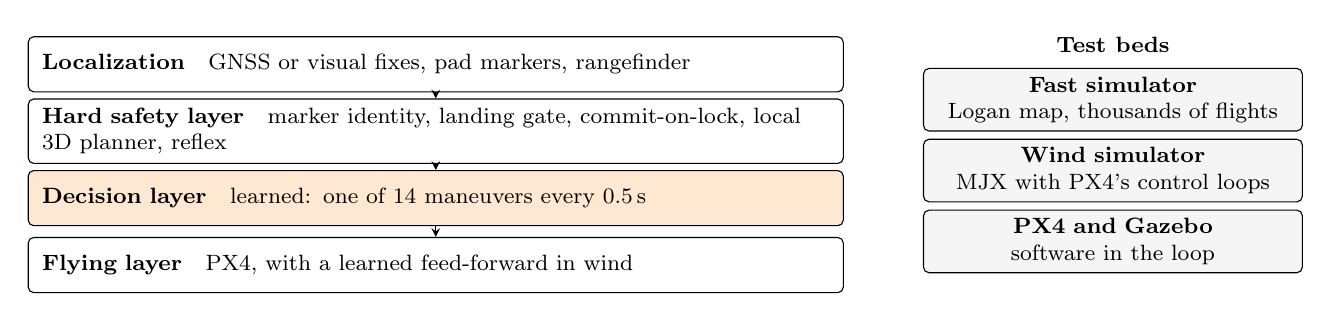
\begin{tikzpicture}[font=\footnotesize, >=stealth,
  layer/.style={draw, rounded corners=2pt, text width=10.0cm, minimum height=7mm, align=left, inner xsep=5pt},
  bed/.style={draw, rounded corners=2pt, text width=4.6cm, minimum height=7mm, align=center, fill=black!4, inner sep=3pt}]
  \node[layer] (loc)  at (0, 0)     {\textbf{Localization}\hspace{1em}GNSS or visual fixes, pad markers, rangefinder};
  \node[layer] (safe) at (0, -0.85) {\textbf{Hard safety layer}\hspace{1em}marker identity, landing gate, commit-on-lock, local 3D planner, reflex};
  \node[layer, fill=orange!18] (dec) at (0, -1.7) {\textbf{Decision layer}\hspace{1em}learned: one of 14 maneuvers every 0.5\,s};
  \node[layer] (fly)  at (0, -2.55) {\textbf{Flying layer}\hspace{1em}PX4, with a learned feed-forward in wind};
  \foreach \a/\b in {loc/safe, safe/dec, dec/fly} \draw[->] (\a.south) -- (\b.north);
  \node[bed] (fast) at (8.6, -0.45) {\textbf{Fast simulator}\\ Logan map, thousands of flights};
  \node[bed] (mjx)  at (8.6, -1.35)  {\textbf{Wind simulator}\\ MJX with PX4's control loops};
  \node[bed] (gz)   at (8.6, -2.25) {\textbf{PX4 and Gazebo}\\ software in the loop};
  \node[font=\footnotesize\bfseries] at (8.6, 0.25) {Test beds};
\end{tikzpicture}
\caption{The landing stack: four layers, one learned decision layer, and the three test beds that run it.}\label{fig:stack}
\end{figure*}


Figure~\ref{fig:stack} shows the stack. Each layer answers one question and hands a smaller problem to the layer below it.

\textbf{Localization.} The drone localizes in two stages (Figure~\ref{fig:pad}(b)). With GNSS available, PX4's estimator (EKF2) fuses it. For the global approach without GNSS, an absolute visual localization module matches the downward camera image against satellite imagery of the suburb. It sends each accepted fix to EKF2 as an auxiliary global position. These fixes are a few meters off, enough to bring the drone to the pad but not to land it.

\textbf{Terminal pad localization.} The delivery pad is a 5~m square mat carrying three ArUco markers \cite{garrido2014} in a row, 1.80, 1.20 and 0.15~m across (Figure~\ref{fig:pad}(a)). The smallest sits at the touchdown point, and the drone reads the largest first and the smallest last. Each readable marker gives a position relative to the pad, and a downward rangefinder gives height. A touchdown error therefore measures this terminal stage, not the satellite-image fixes.

% The delivery pad and the two-stage localization (TikZ), two panels with their labels below. Every size and position is
% make_pad.py's MARKERS and MAT; the radii are the landing tests of gz_learner.py (1.0 m) and wind/gz_windland.py (PAD_R 0.75 m).
\begin{figure*}[t]\centering
\begin{minipage}[b]{0.29\textwidth}\centering
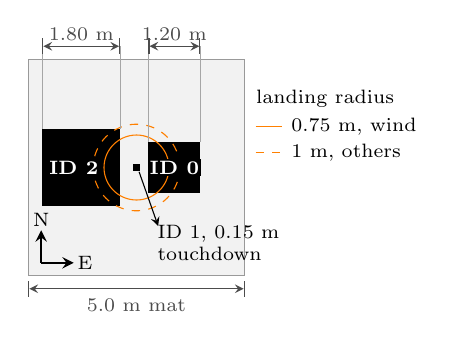
\begin{tikzpicture}[>=stealth, font=\scriptsize, x=0.55cm, y=0.55cm]
  \fill[black!5] (-2.5,-2.5) rectangle (2.5,2.5);
  \draw[black!40] (-2.5,-2.5) rectangle (2.5,2.5);
  \fill (-2.175,-0.9) rectangle (-0.375,0.9);                           % ID 2, 1.80 m, centre x = -1.275
  \fill (0.275,-0.6) rectangle (1.475,0.6);                             % ID 0, 1.20 m, centre x = +0.875
  \fill (-0.075,-0.075) rectangle (0.075,0.075);                        % ID 1, 0.15 m, at the origin
  \draw[orange] (0,0) circle (0.75);
  \draw[orange, dashed] (0,0) circle (1.0);
  \node[white, fill=black, inner sep=0.8pt, font=\scriptsize\bfseries] at (-1.45,0) {ID 2};
  \node[white, fill=black, inner sep=0.8pt, font=\scriptsize\bfseries] at (0.875,0) {ID 0};
  % sizes above the mat, on extension lines from the markers' corners
  \foreach \xa/\xb/\h in {-2.175/-0.375/0.9, 0.275/1.475/0.6} \draw[black!35, very thin] (\xa,\h) -- (\xa,2.8) (\xb,\h) -- (\xb,2.8);
  \draw[|<->|, black!70] (-2.175,2.8) -- node[above=2pt, inner sep=0pt] {1.80 m} (-0.375,2.8);
  \draw[|<->|, black!70] (0.275,2.8) -- node[above=2pt, inner sep=0pt] {1.20 m} (1.475,2.8);
  \draw[->] (0.06,-0.1) -- (0.5,-1.35) node[below right=-2pt, align=left, inner sep=1pt] {ID 1, 0.15 m\\touchdown};
  \draw[->, thick] (-2.2,-2.2) -- (-1.45,-2.2) node[right, inner sep=1pt] {E};
  \draw[->, thick] (-2.2,-2.2) -- (-2.2,-1.45) node[above, inner sep=1pt] {N};
  \draw[|<->|, black!70] (-2.5,-2.8) -- node[below] {5.0 m mat} (2.5,-2.8);
  \node[anchor=west, inner sep=0pt] at (2.75,1.6) {landing radius};
  \draw[orange] (2.75,0.95) -- (3.35,0.95) node[right, black] {0.75 m, wind};
  \draw[orange, dashed] (2.75,0.35) -- (3.35,0.35) node[right, black] {1 m, others};
\end{tikzpicture}\\[3pt]
{\small (a) The pad from above}
\end{minipage}\hfill
\begin{minipage}[b]{0.69\textwidth}\centering
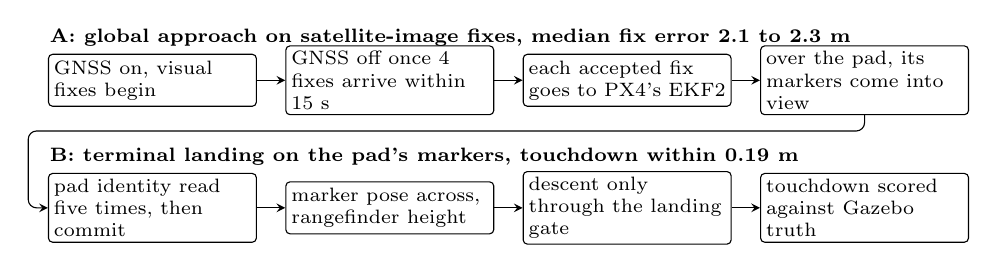
\begin{tikzpicture}[>=stealth, font=\scriptsize, box/.style={draw, rounded corners=1.5pt, text width=2.5cm, align=flush left, inner sep=2pt, minimum height=0.66cm},
                    hd/.style={font=\scriptsize\bfseries, anchor=south west, inner sep=0.5pt}]
  \node[box] (s1) at (0,0.62) {GNSS on, visual fixes begin};
  \node[box, right=0.36cm of s1] (s2) {GNSS off once 4 fixes arrive within 15 s};
  \node[box, right=0.36cm of s2] (s3) {each accepted fix goes to PX4's EKF2};
  \node[box, right=0.36cm of s3] (s4) {over the pad, its markers come into view};
  \node[box] (s5) at (0,-1.0) {pad identity read five times, then commit};
  \node[box, right=0.36cm of s5] (s6) {marker pose across, rangefinder height};
  \node[box, right=0.36cm of s6] (s7) {descent only through the landing gate};
  \node[box, right=0.36cm of s7] (s8) {touchdown scored against Gazebo truth};
  \node[hd] at ([yshift=2pt]s1.north west) {A: global approach on satellite-image fixes, median fix error 2.1 to 2.3 m};
  \node[hd] at ([yshift=2pt]s5.north west) {B: terminal landing on the pad's markers, touchdown within 0.19 m};
  \foreach \a/\b in {1/2, 2/3, 3/4, 5/6, 6/7, 7/8} \draw[->] (s\a) -- (s\b);
  % A to B: down from the last box, back under row A, and in from the left, clear of B's heading
  \draw[->, rounded corners=3pt] (s4.south) -- ++(0,-0.2) -| ([xshift=-0.25cm]s5.west) -- (s5.west);
\end{tikzpicture}\\[3pt]
{\small (b) The two localization stages}
\end{minipage}
\caption{The delivery pad and its two localization stages.}\label{fig:pad}
\end{figure*}


\textbf{Hard safety layer.} Some rules no decider may override, and that is all we mean by hard. The rules act on the same imperfect sensing as the deciders, so they guarantee nothing about a person hidden in fog or a magpie seen late. The drone lands only after it reads the customer's marker identity. Below 6~m it descends only while centered and still over the pad, a condition we call the landing gate. After five reads of its own pad's marker it commits to that pad, a rule we call commit-on-lock. A short loss of sight then means a slow descent at 0.5~m/s instead of a new search. A local 3D planner runs weighted A* over the surveyed map and a voxel map from the forward depth camera. It keeps 2~m from anything blocked and pays a cost for passing within 5~m. Between decisions, a reflex applies the rule's magpie dodge every 0.25~s. The fast simulator flies thousands of drones at once and runs a lighter version of this layer. It checks the map and voxel map ahead instead of running A*. It models no wind and counts any touchdown within 1~m of the pad center, so it has no landing gate.

\textbf{Decision layer.} Every 0.5~s one decider picks one of 14 candidate velocity commands. Two are the rule's command and the guidance command it starts from, which heads for the pad. The guidance command also appears turned $45^\circ$ or $90^\circ$ either way, reversed, at half speed, held level and climbing. The other four are landing anyway, hovering, climbing straight up and flying away from the helipad. Every candidate is capped at 8~m/s across, 3~m/s up and 2.5~m/s down. The rule, both planners and the learner choose from the same list, so any difference between them comes from the decision alone.

\textbf{Flying layer.} PX4 tracks the chosen velocity. In the wind study a flying learner adds an acceleration feed-forward of at most 3~m/s$^2$ per axis to that velocity setpoint.

\subsection{Three Test Beds}

\textbf{Fast simulator.} Thousands of deliveries advance in lock-step on the GPU in 0.25~s steps, with a 300~s limit per flight. The map covers 4~km by 4~km of Logan at 1~m resolution, rebuilt from the 2023 airborne LiDAR survey (Figure~\ref{fig:world}). It holds 1,324 candidate pads and a hospital helipad. Each flight starts 50~m up, at most 1~km from its pad in the direction of the depot. PX4's velocity response enters as first-order lags that we measured on PX4, 0.69~s horizontal and 0.23~s vertical. An air ambulance arrives on half the flights, and in the world we report it always comes from the north-west. Up to six other delivery drones fly between the depot and customers, and people and cars appear near the pad.

We apply three drone safety rules that the Civil Aviation Safety Authority (CASA) sets for recreational flying \cite{casa2026}. They serve as safety constraints in the simulation, not as an assessment of regulatory compliance for commercial delivery. The drone stays below 120~m and at least 30~m from people, and never flies over a person. Within 1.4~km of a helicopter landing site, it moves away from a helicopter that is nearby, taking off or landing. A near mid-air collision (NMAC) with the air ambulance follows ASTM F3442 \cite{astm2023}, which covers encounters with crewed aircraft: 152~m horizontally and 30~m vertically. We assume a 30~m separation between drones, since we found no CASA figure for it. A clean delivery is a touchdown on the right pad with no crash, no NMAC and no rule broken during the flight.

\begin{figure}[t]\centering\includegraphics[width=0.76\linewidth]{world}
\caption{Logan from the 2023 LiDAR survey.}\label{fig:world}\end{figure}

We test four conditions. Clear is the world as described. Unmapped adds tall structures that the survey does not contain, such as cranes, which the drone senses only with its depth camera. Fog covers every flight. We measured in Gazebo how often the drone reads the marker through fog at each height, relative to calm air. The share falls from every frame at 5~m to 36\% of frames at 46~m. Fog hides people as well.

Magpie adds a territorial Australian magpie near half the pads. It attacks from behind, keeps steering through its dive with turns of up to 20~m/s$^2$, and commits to its path 0.3~s before contact. The drone knows the magpie either exactly or through a model of a six-camera rig, its small detector and a tracker, calibrated on Gazebo renders of that rig.

\textbf{Wind simulator.} For wind we need flight dynamics, so we model the x500 quadrotor in MuJoCo \cite{todorov2012}, run with MuJoCo XLA (MJX) on the GPU. The drone is a 2.584~kg rigid body with Gazebo's motor and propeller-drag model. We emulate PX4's velocity, attitude and rate loops and its control allocation with PX4's default gains.

We report the mean wind 10~m above ground as W10. The same wind drives MJX and a Gazebo plugin we wrote: a logarithmic profile, turbulence in the low-altitude form of MIL-F-8785C \cite{milf8785c}, and one-minus-cosine gusts. The specification scales turbulence by the wind at 20~ft, and we scale it by W10. The two simulators agree closely. For a 0 to 8~m/s velocity step, 63\% of the response takes 0.85~s in Gazebo and 0.80~s in MJX. Hovering in a steady 15.8~m/s wind, the drone tilts 22.5$^\circ$ in Gazebo and 22.6$^\circ$ in MJX.

The wind task starts 30~m up and 15 to 25~m from a back-yard pad. A house stands 2.5 to 8~m away, and a tree stands beside the pad in 60\% of yards. A landing counts when the drone touches down within 0.75~m of the center, sinking slower than 1~m/s and sliding slower than 0.5~m/s. Within 0.35~m of the house or tree counts as a crash, any other touchdown as hard or off the pad, and 90~s aloft as a timeout.

\textbf{PX4 and Gazebo.} The last test bed runs PX4 v1.16.2 in software-in-the-loop with Gazebo \cite{koenig2004}. The x500 model carries our camera rig. It has a forward stereo depth camera with a color sensor, wide cameras to the left, right and rear, and a landing camera on a gimbal. One variant adds a wide camera looking up. The suburb, pads, crane and magpie are the fast simulator's, rebuilt as Gazebo worlds.

\section{Measuring Before Training}\label{sec:method}

\textbf{A ladder of deciders without learning.} For every condition we run three deciders on the same 4,096 test flights, which share every random draw. The rule is a hand-written reactive decider with fixed margins around people, aircraft and birds. The same-sensor planner rolls each of the 14 candidates forward for 20~s against its predictions of every intruder it has sensed. It extends each track in a straight line at its sensed velocity and replans every 0.5~s. Its cost adds progress over 5~s, predicted violations over 20~s, and a deadline term. The deadline term charges any overrun of the 300~s flight limit that a plan implies, so the 20~s window still weighs the rest of the flight. The planner comes in two forms: the shield flies the rule's command unless the forecast shows a violation, and then takes the least risky alternative. The safe planner never accepts a predicted violation when a safe candidate exists, and among the safe candidates takes the fastest.

We report the better of the two on the test flights as the best same-sensor planner. That choice can only flatter the planner, so the learner's measured gain over it is, if anything, too small. The privileged planner uses the same two forms, but reads every intruder's true future from the simulator. The gap from the rule to the best same-sensor planner is room for better decisions. The gap from there to the privileged planner is room for better information. Both gaps are measured with planners that choose among 14 constant commands over 20~s. They show room within that class of planner, not the most any decider could gain, and the privileged planner is a reference, not a ceiling.

\textbf{Paired statistics.} Because all deciders fly the same flights, we compare them flight by flight. A difference is the mean of the per-flight differences in percentage points. For one trained learner, the 95\% interval is 1.96 standard errors over the test flights, which leaves out training variation. The three seeds share the test flights, so their spread leaves out flight variation. For the mean over seeds we combine the widest per-seed interval with a Student's $t$ interval over the seed means, as the root of their summed squares. We choose checkpoints on 2,048 separate validation flights and never on the test flights.

\textbf{Learned decision layer.} The learner sees its own state, the pad, its helipad duty, and the tracks of every intruder its sensors report. The tracks fill fixed slots, nearest first, and an empty slot is set to zero. It also sees what the same-sensor planner concluded about each candidate: its 20~s violation forecast, its progress over 5~s, its deadline overrun, and its pick. We added this input because of an earlier version of the fast simulator. There, PPO from scratch reached 91.8\% clean deliveries, below the rule, and a copy of the planner in the same network reached 94.1\% and no further. Table~\ref{tab:learner} lists the inputs, the network and the training settings.

Training starts with a copy of the shield planner, taught by dataset aggregation (DAgger) \cite{ross2011}, and continues with PPO. Before PPO, the copy's top choice scored exactly the planner's rate of clean deliveries on the validation flights, in every seed and condition. A gain over the copied planner is therefore what PPO added. The reward is $+1$ for a clean delivery, $-1$ for a crash, $-1$ per NMAC, $-0.25$ per second of rule violation and $-0.001$ per decision. Waiting 300~s therefore costs less than a clean delivery is worth. Each seed trains for 200 generations of 2,048 flights, 409,600 flights in all. We train three seeds per condition.

\begin{table}[t]
\centering\footnotesize
\setlength{\tabcolsep}{4pt}
\caption{The learned decision layer and its training in the fast simulator.}
\label{tab:learner}
\begin{tabular}{@{}ll@{}}
\toprule
Inputs & 221, magpie 228 \\
\quad own state, pad, helipad & 7, 5, 5 \\
\quad intruder slots & $15 \times 7$, magpie $16 \times 7$ \\
\quad candidates, pad blocked & $14 \times 3$, 1 \\
\quad planner's view & $14 \times 4$ \\
\quad scaling & fixed constants \\
Policy, value networks & separate, $2 \times 256$ ReLU \\
Parameters & 249,103, magpie 252,687 \\
Action at test time & sampled, exact repeats masked \\
\midrule
Imitation (DAgger) & 3 rounds of 2,048 flights \\
\quad planner flying & 100, 50, 0\% of decisions \\
\quad decisions labeled & 2.2 to 2.3 million \\
\quad optimizer & Adam $10^{-3}$, 8 epochs a round \\
\quad label smoothing & 0.05 \\
PPO generations & 200 of 2,048 flights \\
\quad optimizer & Adam $10^{-4}$, 4 epochs \\
\quad minibatch & 32,768 decisions \\
\quad clip, $\gamma$, GAE $\lambda$ & 0.2, 0.997, 0.95 \\
\quad entropy bonus & 0.002 falling to 0.0002 \\
\quad value weight, grad.\ clip & 0.5, 0.5 \\
\quad value trained alone & first 5 generations \\
Validation check & every 10 generations \\
PPO time per seed & 1.1 to 2.0~h (RTX 5070) \\
\bottomrule
\end{tabular}
\end{table}


\textbf{Learned flying and deciding in wind.} Here the rule is the landing part of the stack. It approaches the pad, descends at 1.5~m/s above 8~m and 0.8~m/s below, and below 6~m descends only through the landing gate. The wind learner acts through what PX4 accepts over MAVLink. Its flying output adds an acceleration feed-forward to the rule's velocity setpoint. Its deciding output picks the vertical action every 0.04~s among the rule's own, down at 1.5~m/s, down at 0.6~m/s, hold and up at 1~m/s. Training uses PPO in JAX on 4,096 drones at once, with a wind curriculum. The curriculum starts at 4~m/s and adds 1~m/s once 95\% of flights in the top band land, or after 150 training rounds at one level.

The flying learner keeps the rule's decisions and learns only the feed-forward. PX4's velocity integrator cancels a steady push, so we remove the slow part of the feed-forward with a 4~s high-pass filter. The crash-priced decider learns only the vertical action, on top of a frozen flying learner. A crash and a hard or off-pad touchdown each cost $-100$. A potential-based term rewards progress toward the pad with the learner's own discount of 0.9998. With 0.997, which we first used, hovering near the start earned about as much as landing. We train eight seeds of the flying learner and three of the decider, and evaluate each on 1,024 paired flights per wind speed.

\section{Results in the Fast and Wind Simulators}

\begin{table*}[t]
\centering\small
\setlength{\tabcolsep}{5pt}
\caption{Clean deliveries (\%) on the same 4,096 test flights per condition. Shield and safe: the same-sensor planners, the better in bold. Learner: mean (range) of three seeds. Gains: paired, mean of three seeds, $\pm$ a 95\% interval over seeds and flights (Section~\ref{sec:method}). Gains over the safe planner come from a second evaluation of the same learners on the same flights.}
\label{tab:ladder}
\begin{tabular}{lcccccccc}
\toprule
 & & \multicolumn{2}{c}{Same-sensor planner} & Privileged & & \multicolumn{2}{c}{Learner's gain over} \\
\cmidrule(lr){3-4}\cmidrule(lr){7-8}
Condition & Rule & Shield & Safe & planner & Learner & copied shield & best same-sensor \\
\midrule
Clear & 93.7 & \textbf{94.5} & 94.3 & 95.4 & 96.4 (96.3--96.4) & $+1.9 \pm 0.5$ & $+1.9 \pm 0.5$ \\
Unmapped structures & 93.3 & 94.0 & \textbf{94.3} & 94.4 & 96.0 (95.9--96.1) & $+2.0 \pm 0.7$ & $+1.9 \pm 0.8$ \\
Fog & 68.8 & \textbf{71.9} & 69.3 & 95.7 & 86.4 (84.8--88.8) & $+14.6 \pm 5.4$ & $+14.6 \pm 5.4$ \\
Magpie, known exactly & 79.1 & \textbf{78.7} & 77.7 & 78.9 & \multicolumn{3}{c}{not trained (no room)} \\
Magpie, camera rig & 72.6 & 69.8 & \textbf{73.5} & 75.1 & 77.5 (77.1--77.7) & $+7.7 \pm 1.7$ & $+4.1 \pm 2.2$ \\
\bottomrule
\end{tabular}
\end{table*}


\subsection{Room for Better Decisions}

Table~\ref{tab:ladder} gives the ladder and the learners. In clear weather the three deciders without learning span 1.8 points, from the rule's 93.7\% to the privileged planner's 95.4\%. Unmapped structures cost the rule 0.3 points and leave the privileged planner only 0.1 points above the best same-sensor planner. Fog is different. The best same-sensor planner reaches 71.9\% and the privileged planner 95.7\%, a gap of 23.8 points, which Section~\ref{sec:method} defines as room for better information. Handed the magpie's true position, the rule already matches both planners (79.1\% against 78.7\% and 78.9\%), so the ladder shows no room for better decisions. Through the camera rig the room returns: 72.6\% for the rule, 73.5\% for the best same-sensor planner and 75.1\% for the privileged planner.

\subsection{What the Learner Added}

\begin{figure*}[t]\centering
\begin{minipage}[b]{0.6\textwidth}\centering\includegraphics[width=\linewidth]{learning_a}\\[2pt]{\small (a) Validation during training}\end{minipage}\hfill
\begin{minipage}[b]{0.38\textwidth}\centering\includegraphics[width=\linewidth]{learning_b}\\[2pt]{\small (b) Test gain over the copied planner}\end{minipage}
\caption{The learners in training and on the test flights, three seeds per condition.}\label{fig:learning}\end{figure*}

The learner beat the planner it copied in every condition and every seed, and each seed's paired interval excludes zero (Table~\ref{tab:ladder}, Figure~\ref{fig:learning}). The copied shield planner is also the best same-sensor planner in clear weather and fog. With unmapped structures and with the magpie seen through the rig, the safe planner does better. There we compared the same learners with it in a second evaluation on the same test flights, paired flight by flight. Against the best same-sensor planner, the gain is largest where information is missing: 14.6 points in fog and 4.1 with the magpie seen through the rig. It is 1.9 points in clear weather and 1.9 with unmapped structures, and every seed's interval excludes zero in all four conditions. With the magpie, the seeds range from 3.5 to 4.8 points, each with a 95\% interval of about $\pm 1.5$. The gain of 7.7 points over the copied planner is larger because that planner reaches only 69.8\% there, below the safe planner's 73.5\%. In three conditions the learner also beats the privileged planner, which still plans over only 14 constant commands.

The first failure reason of each flight shows how the learner gained. In fog, flights that ended with the drone over a person fell from 24.5\% for the copied planner to 6.8\% for the learner. Flights that came within 30~m of a person rose from 0.0\% to 4.1\%. With the magpie seen through the rig, strikes fell from 22.7\% of all flights to 17.9\%. In clear weather the learner mainly timed out less often while people stood at the pad, on 1.8\% of flights against the planner's 2.8\%.

\begin{table}[!tb]
\centering\small
\setlength{\tabcolsep}{3pt}
\caption{Landing in gusty wind. MJX: landed \% (crashed \%) on 1,024 paired flights per wind speed, learners as the median over seeds (number of seeds in brackets). Gazebo: landed of flown on the same 20 yards and gusts, crashes in brackets where any. A rate from 1,024 flights has a 95\% interval of at most $\pm 3.1$ points. Two rule flights, at 15 and 18~m/s, stopped on a simulator fault and left no record.}
\label{tab:wind}
\begin{tabular}{lccc}
\toprule
W10 (m/s) & 12 & 15 & 18 \\
\midrule
\multicolumn{4}{l}{\textit{MJX}} \\
Rule & 100 (0.0) & 77.9 (0.0) & 5.6 (0.1) \\
Flying learner (8) & 100 (0.0) & 99.1 (0.0) & 50.7 (0.1) \\
Crash-priced decider (3) & 99.0 (0.0) & 98.6 (0.1) & 96.2 (1.0) \\
\midrule
\multicolumn{4}{l}{\textit{Gazebo with PX4}} \\
Rule & 19/20 & 12/19 & 0/19 \\
Flying learner, s.~0 & 20/20 & 18/20 & 6/20 \\
Flying learner, s.~1 & 20/20 & 19/20 & 5/20 \\
Crash-priced decider, s.~0 & 18/20 & 19/20 & 18/20 \\
\bottomrule
\end{tabular}
\end{table}


\subsection{Knowing the Magpie}

How the drone knows the magpie sets the strike rate more than the decider does. With the rule deciding, 27.7\% of magpie flights end in a strike when the drone knows the magpie exactly, and 38.9\% through the rig. The rate is 41.6\% when the rig sees only half as far, and 45.1\% with only the drone's forward and landing cameras. Better deciders move these figures by a few points at most. Through the rig the best same-sensor planner is struck on 38.8\% of magpie flights and the privileged planner on 37.7\%.

The Gazebo flights use a newer rig on the frame, with YOLO26n \cite{sapkota2025} fine-tuned on 4,115 labeled renders over plain ground and 4,611 over photographic ground. On renders from drone positions unseen in training, it found 89\% of magpies over plain ground (511 pictures) and 81\% over photographic ground (577), at a 0.5 threshold. Before the photographic renders, it boxed tree crowns and roofs 0.57 times per picture, and after them 0.002 times. It found 85 to 86\% of magpies within 20~m and 59\% at 45 to 70~m.

\subsection{Landing in Gusty Wind}

The rule never crashes in wind (Table~\ref{tab:wind}). It lands every flight up to a W10 of 12~m/s, 77.9\% at 15~m/s and 5.6\% at 18~m/s. Almost all its failures are timeouts. The flying learner keeps the rule's decisions. It lands 99.1\% at 15~m/s (98.6 to 99.4\% over eight seeds) and 50.7\% at 18~m/s (43.8 to 54.9\%). It crashes on at most 0.5\% of flights at any speed up to 20~m/s.

At 18 and 20~m/s the crash-priced decider lands more flights than the flying learner and crashes more often. It lands 96.2\% at 18~m/s (93.8 to 96.2\%) but crashes on 1.0\% (0.8 to 3.0\%), and at 20~m/s it lands 78.5\% and crashes on 6.5\%. The prices matter. With the earlier discount of 0.997, $-100$ for a crash and $-30$ for a hard touchdown gave a median of 87.3\% landed at 18~m/s and 3.3\% crashed. One decider priced at $-15$ and $-10$ landed 69.1\% and crashed on 11.7\%.

The Gazebo flights on 20 of the same yards, with identical gusts, keep the order. At 15~m/s the rule landed 12 of 19 flights and the two flying learners 18 and 19 of 20. At 18~m/s the rule landed none of 19 and the flying learners 6 and 5. The crash-priced decider landed 18 of 20, with no crash. Flight by flight at 18~m/s, the decider landed 17 flights that the rule did not, and the rule landed none that the decider missed. A two-sided sign test gives $p < 0.001$.

An earlier decider, trained with the 0.997 discount and $-100$ for a hard touchdown, landed 92.1\% at 18~m/s in MJX but alternated between climbing and descending. In Gazebo at 9~m/s it reversed 1.7 times per second and landed 16 of 20, and its four hard landings touched down at 1.06 to 1.15~m/s. One seed of the crash-priced decider reversed 2.2 times per second in MJX at 9~m/s, so we count reversals before any Gazebo flight. The seed we flew reversed at most 0.34 times per second in Gazebo.

\section{PX4 Software-in-the-Loop Flights in Gazebo}

\begin{figure*}[t]\centering
\begin{minipage}[b]{0.14\textwidth}\centering\includegraphics[width=\linewidth]{gazebo_a.jpg}\\[2pt]{\small (a) Thick fog}\end{minipage}\hspace{2mm}%
\begin{minipage}[b]{0.245\textwidth}\centering\includegraphics[width=\linewidth]{gazebo_b.jpg}\\[2pt]{\small (b) Voxels and planned path}\end{minipage}\hspace{2mm}%
\begin{minipage}[b]{0.245\textwidth}\centering\includegraphics[width=\linewidth]{gazebo_c.jpg}\\[2pt]{\small (c) Magpie near the drone}\end{minipage}\hspace{2mm}%
\begin{minipage}[b]{0.245\textwidth}\centering\includegraphics[width=\linewidth]{gazebo_d.jpg}\\[2pt]{\small (d) Pad at touchdown}\end{minipage}
\caption{Frames from the PX4 flights in Gazebo.}\label{fig:gazebo}\end{figure*}

\textbf{Weather.} With GNSS, the rule deciding and the marker guiding touchdown, we flew ten flights in each of five skies on the same seeds (Figure~\ref{fig:gazebo}(a)). Wind of 7~m/s with gusts to about 10~m/s cost no landing. Mist and thick fog cost one and three landings. Every failure was a safe abort: the drone lost its marker in a fog patch and searched away, once only 0.68~m from its own pad. With commit-on-lock, mist and fog both landed 10 of 10, and the median miss was 0.33 to 0.37~m in every sky. The marker was first read at about 51~m in every sky.

\textbf{Unmapped crane.} We placed a crane at ten positions on the approach and flew the rig with GNSS. A planner that knew only the survey crashed into the crane in 8 of 10 flights. A planner that looked ahead on the voxel map passed all ten but came within 0.99~m. The rule with the local 3D planner passed all ten, never closer than 2.59~m (median 3.42~m).

\textbf{Magpie with the live detector.} With GNSS, the drone knew the magpie only through the up-camera rig's live detector and tracker. The planner and a learner trained with that rig's model each landed 5 of 9 flights. These flights span three revisions of the landing code, so they show only that detection works in the loop.

\begin{table*}[t]
\centering\small
\setlength{\tabcolsep}{5pt}
\caption{PX4 flights in Gazebo with GNSS denied, the last flight of each scenario. Errors against Gazebo's truth, median / 90th percentile. Miss: touchdown distance from the pad center. Flying learner: wind seed 0. Learner: trained with the up-camera rig's model, not Table~\ref{tab:ladder}'s, flying the probability-weighted mean of its commands.}
\label{tab:gnssfree}
\begin{tabular}{llcccc}
\toprule
Scenario & Decider & GNSS off (s) & Visual fix error (m) & PX4 error (m) & Miss (m) \\
\midrule
Calm & Rule & 110 & 2.13 / 4.95 & 2.32 / 3.89 & 0.06 \\
Wind, W10 9~m/s & Flying learner & 117 & 2.12 / 4.71 & 1.71 / 6.68 & 0.19 \\
Crane on the route & Rule, local 3D planner & 117 & 2.28 / 5.12 & 1.85 / 3.89 & 0.04 \\
Magpie & Learner & 116 & 2.21 / 5.12 & 1.67 / 3.55 & 0.04 \\
Magpie, up camera added & Learner & 116 & 2.17 / 5.11 & 1.44 / 3.52 & 0.08 \\
Mission to another pad & Rule & 107 & 2.26 / 5.17 & 3.13 / 4.82 & 0.05 \\
\bottomrule
\end{tabular}
\end{table*}


\textbf{GNSS-denied deliveries.} Table~\ref{tab:gnssfree} lists six flights with GNSS denied over the suburb, the last flight of each scenario. The drone cruised at 75~m on a planned route, and we denied GNSS once PX4 had accepted four visual fixes within 15~s. The visual localization module matched each downward image against satellite imagery captured in 2021. The simulated ground and roofs carried a 2023 capture of the same area, so the map never equals what the camera sees. Per flight, the median fix error was 2.1 to 2.3~m, the 90th percentile 4.7 to 5.2~m, and 97.8 to 98.5\% of fixes fell within 10~m. PX4's fused position had a median error of 1.4 to 3.1~m. On the laptop that ran the simulation, a visual fix was ready a median of 11 to 41~ms after its image was taken. Once the pad's markers were readable they took over, and every flight landed within 0.19~m of the pad center. The touchdown accuracy therefore comes from the markers, and the visual fixes had to bring the drone close enough to read them.

These six flights are integration demonstrations, not a landing rate. Before them, and after short pipeline tests, we flew 18 development flights in the same scenarios. Six failed: a hard landing, a crash in wind, lost visual fixes, a crash into the crane, a timeout and a landing 659~m off the pad. Each led to a fix: a downward rangefinder, marker fixes kept until touchdown with an outlier check, and one simulator per computer. Weighted A* fixed the crane crash by cutting a plan from about 2~s to 17~ms.

We then repeated the calm flight ten times on one frozen code version, changing only the landing heading. All ten landed, 0.04 to 0.07~m from the pad center, with GNSS denied for 109 to 130~s and PX4's median error 2.0 to 2.9~m. As with the weather flights, 10 of 10 shows only that the landing rate exceeds 69\% at 95\% confidence, and calm air is the easiest case.

The rig's cameras and the detector shared one laptop GPU (RTX 5070), and we slowed each magpie landing to a tenth of real time for the detector. Timed separately on that GPU, the detector took a median of 54 to 65~ms per set of four or five pictures. The slowest set took 157~ms, inside the 0.25~s reflex period. It ran beside the slowed simulation without pausing it, so its delay cost the drone a tenth of the simulated time it would in real time. These flights validate the software integration, not real-time operation on a drone's own computer.

\section{Discussion}

\textbf{Where learning paid.} Learning paid where the sensors miss something that matters, such as people hidden by fog or a magpie seen late. It also paid where a rule's safety gate rarely opens, as in strong gusts. Where the drone already knew enough, as with the magpie known exactly, a rule with a fast reflex left nothing to learn. In clear weather the learner added about two points, mostly by managing time around people at the pad. Learning to fly under the rule's decisions never raised crashes above 0.5\%, while learning to decide traded timeouts for crashes at a rate set by the crash price. For that reason we keep the hard rules outside every learned layer.

\begin{table}[t]
\centering\footnotesize
\setlength{\tabcolsep}{4pt}
\caption{Learner's gain in points over the copied (cop.) and the best same-sensor planner, one assumption changed at a time, learners not retrained, mean of three seeds. Defaults: people leave within 30--240~s, 300~s limit, drones 30~m apart, magpie commits 0.3~s before contact, rig range 40~m. The first row is a second evaluation, within 0.2 points of Table~\ref{tab:ladder}.}
\label{tab:sens}
\begin{tabular}{@{}lcccccc@{}}
\toprule
 & \multicolumn{2}{c}{Clear} & \multicolumn{2}{c}{Fog} & \multicolumn{2}{c}{Magpie, rig} \\
\cmidrule(lr){2-3}\cmidrule(lr){4-5}\cmidrule(lr){6-7}
Assumption changed & cop. & best & cop. & best & cop. & best \\
\midrule
As in Table~\ref{tab:ladder} & 1.8 & 1.8 & 14.4 & 14.4 & 7.8 & 4.1 \\
Leave 10--120~s & 2.0 & 1.9 & 12.4 & 12.4 & 8.2 & 4.2 \\
Leave 60--480~s & 1.5 & 1.2 & 6.5 & 6.5 & 6.2 & 3.2 \\
Limit 200~s & 2.2 & $-0.4$ & 9.2 & 6.9 & 11.4 & 4.4 \\
Limit 400~s & 0.8 & 0.8 & 14.7 & 14.7 & 5.8 & 3.7 \\
Drones 50~m & 1.4 & 1.4 & 14.1 & 14.1 & 7.3 & 3.9 \\
Commit 0.1~s & -- & -- & -- & -- & 7.9 & 3.9 \\
Commit 0.5~s & -- & -- & -- & -- & 6.7 & 3.2 \\
Rig range half & -- & -- & -- & -- & 7.6 & 4.3 \\
\bottomrule
\end{tabular}
\end{table}


\textbf{Limitations.} Every result here comes from simulation. The fast simulator rests on assumptions that move its numbers, from when people leave the pad to how far the rig sees. We changed each assumption alone, 18 variations in all (Table~\ref{tab:sens}), and evaluated the trained learners again without retraining.

Every decider's clean deliveries moved by up to 33 points, yet the learner beat the planner it copied in every variation and every seed. The gain stayed at least 5.8 points in fog and with the magpie and at most 2.2 in clear weather. Against the best same-sensor planner it stayed at least 6.5 points in fog and 3.2 with the magpie. In one clear-weather variation, a 200~s limit, the learner fell 0.4 points below the safe planner.

The air ambulance always arrives from the north-west. In earlier clear-weather runs with the visual localization module's position errors instead of GNSS, we also let it arrive from any direction. The learner's gain over its copied planner was then 2.4 to 2.7 points, against 1.9 to 2.1 from the north-west. The fast simulator's rig model scatters false alarms at random, while the live detector's false boxes gathered on trees and roofs. Its fog model comes from Gazebo's rendering of the marker, not from measurement outdoors. The body drag in both wind simulators uses assumed coefficients. The PX4 evidence is thin where it matters most: ten GNSS-denied flights in calm air but one in each harder scenario, and nine live magpie flights per decider. The privileged planner is a reference, not a bound, since the learner beat it in three conditions.

\textbf{Next steps.} Like VO-Safe RL \cite{lin2024vosafe}, we plan to give the decision layer the health of its own localization, with a penalty for losing it. The health will come from the visual fixes and PX4's optical flow. We will add drones that cross the landing area and moving objects the detector never saw, and measure the room for better decisions before training.

\section{Conclusion}

We built a hierarchical landing stack for delivery drones and asked, condition by condition, where a learned decision layer pays for itself. In simulation, against the best same-sensor planner, learning added 14.6 points of clean deliveries in fog, 4.1 against a magpie seen through cameras and 1.9 elsewhere. Against the planner it started from, the magpie gain was 7.7 points. A learned flying layer also landed in gusts that the rule waited out. With GNSS denied in PX4 software-in-the-loop, visual fixes brought the drone to the pad, and the pad's markers guided it to within 0.19~m of the center. We will release the simulation code base on GitHub, together with videos of the simulated flights.

\section*{Acknowledgments}

The simulation, training and analysis code was written with the help of Claude (Anthropic), used through Claude Code. The authors designed the experiments, checked the code's outputs against every result reported here, and take full responsibility for the work.


\bibliographystyle{named}
\bibliography{refs}

\end{document}
